% THIS IS SIGPROC-SP.TEX - VERSION 3.1
% WORKS WITH V3.2SP OF ACM_PROC_ARTICLE-SP.CLS
% APRIL 2009
%
% It is an example file showing how to use the 'acm_proc_article-sp.cls' V3.2SP
% LaTeX2e document class file for Conference Proceedings submissions.
% ----------------------------------------------------------------------------------------------------------------
% This .tex file (and associated .cls V3.2SP) *DOES NOT* produce:
%       1) The Permission Statement
%       2) The Conference (location) Info information
%       3) The Copyright Line with ACM data
%       4) Page numbering
% ---------------------------------------------------------------------------------------------------------------
% It is an example which *does* use the .bib file (from which the .bbl file
% is produced).
% REMEMBER HOWEVER: After having produced the .bbl file,
% and prior to final submission,
% you need to 'insert'  your .bbl file into your source .tex file so as to provide
% ONE 'self-contained' source file.
%
% Questions regarding SIGS should be sent to
% Adrienne Griscti ---> griscti@acm.org
%
% Questions/suggestions regarding the guidelines, .tex and .cls files, etc. to
% Gerald Murray ---> murray@hq.acm.org
%
% For tracking purposes - this is V3.1SP - APRIL 2009

\documentclass{acm_proc_article-sp}

\usepackage{graphics}
\begin{document}

\title{Coloured Petri Nets: A Graphical Language for Formal Modelling and Validation of Concurrent Systems}
\subtitle{}

%\titlenote{A full version of this paper is available as
%\textit{Author's Guide to Preparing ACM SIG Proceedings Using
%\LaTeX$2_\epsilon$\ and BibTeX} at
%\texttt{www.acm.org/eaddress.htm}}}
%
% You need the command \numberofauthors to handle the 'placement
% and alignment' of the authors beneath the title.
%
% For aesthetic reasons, we recommend 'three authors at a time'
% i.e. three 'name/affiliation blocks' be placed beneath the title.
%
% NOTE: You are NOT restricted in how many 'rows' of
% "name/affiliations" may appear. We just ask that you restrict
% the number of 'columns' to three.
%
% Because of the available 'opening page real-estate'
% we ask you to refrain from putting more than six authors
% (two rows with three columns) beneath the article title.
% More than six makes the first-page appear very cluttered indeed.
%
% Use the \alignauthor commands to handle the names
% and affiliations for an 'aesthetic maximum' of six authors.
% Add names, affiliations, addresses for
% the seventh etc. author(s) as the argument for the
% \additionalauthors command.
% These 'additional authors' will be output/set for you
% without further effort on your part as the last section in
% the body of your article BEFORE References or any Appendices.

\numberofauthors{2} %  in this sample file, there are a *total*
% of EIGHT authors. SIX appear on the 'first-page' (for formatting
% reasons) and the remaining two appear in the \additionalauthors section.
%
\author{
% You can go ahead and credit any number of authors here,
% e.g. one 'row of three' or two rows (consisting of one row of three
% and a second row of one, two or three).
%
% The command \alignauthor (no curly braces needed) should
% precede each author name, affiliation/snail-mail address and
% e-mail address. Additionally, tag each line of
% affiliation/address with \affaddr, and tag the
% e-mail address with \email.
%
% 1st. author
\alignauthor
Kurt Jensen\\
       \affaddr{Computer Science Department}\\
       \affaddr{Aarhus University, Denmark}\\
       \email{kjensen@cs.au.dk}
% 2nd. author
\alignauthor
Lars M. Kristensen\\
       \affaddr{Department of Computing}\\
       \affaddr{Bergen University College, Norway}\\
       \email{lmkr@hib.no}
}

\maketitle
\begin{abstract}

Coloured Petri Nets (CPNs) combine Petri nets with a programming
language to obtain a scalable formal modelling language for concurrent
systems. Petri nets provide the formal foundation for modelling
concurrency and synchronisation, and a programming language provides
the primitives for modelling data manipulation and creating compact
and parameterisable models. We provide an example driven introduction
to the syntactical and semantical constructs of the CPN modelling
language, and briefly surveys how quantitative and qualitative
behavioural properties of CPN models can be validated using
simulation-based performance analysis and explicit state space
exploration. In addition, we give a brief overview of CPN Tools which
provide tool support for the practical use of CPNs, and provide
pointers to significant example where CPNs and the supporting computer
tool has been put into practical use. As we proceed, we highlight the
historical developments that paved the way for the CPN modelling
language.

\end{abstract}

% A category with the (minimum) three required fields
\category{H.4}{Information Systems Applications}{Miscellaneous}
%A category including the fourth, optional field follows...
\category{D.2.8}{Software Engineering}{Metrics}[complexity measures, performance measures]

\terms{Theory}

\keywords{TODO} % NOT required for Proceedings

\section{Introduction}

REST OF THE FIRST PAGE. MAYBE IT IS OVERKILL TO GIVE AN OVERVIEW OF
THE PAPER AT THE END OF THE INTRODUCTION. PERHAPS WE ALSO NEED TO
RELATE OTHER CLASSICAL LANGUAGES (State Charts, SDL).

\section{An Example CPN Model}

\begin{figure*}[t]
\centering
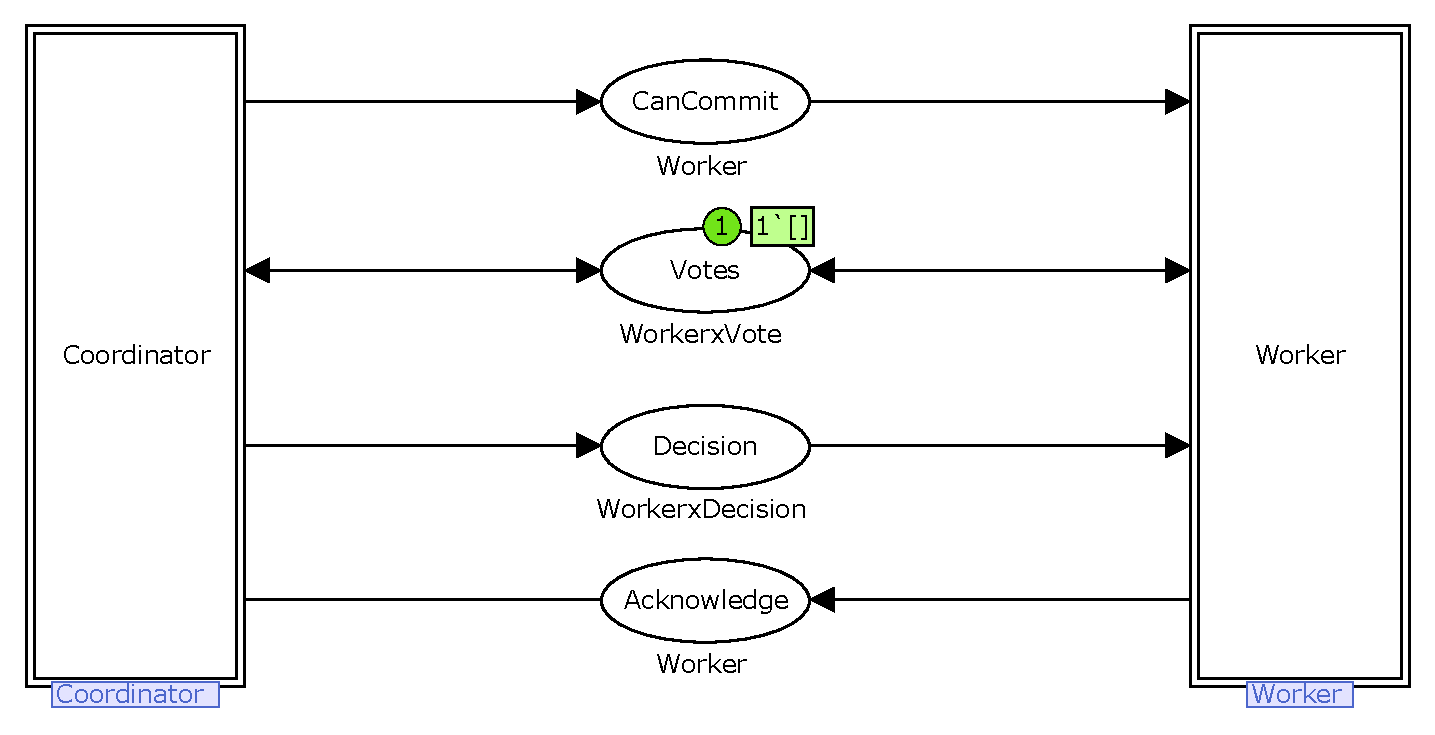
\includegraphics[width=15cm]{figures/Commit.eps}
\caption{The top-level Commit module of the CPN model.}
\end{figure*}

\begin{figure}[t]
\centering
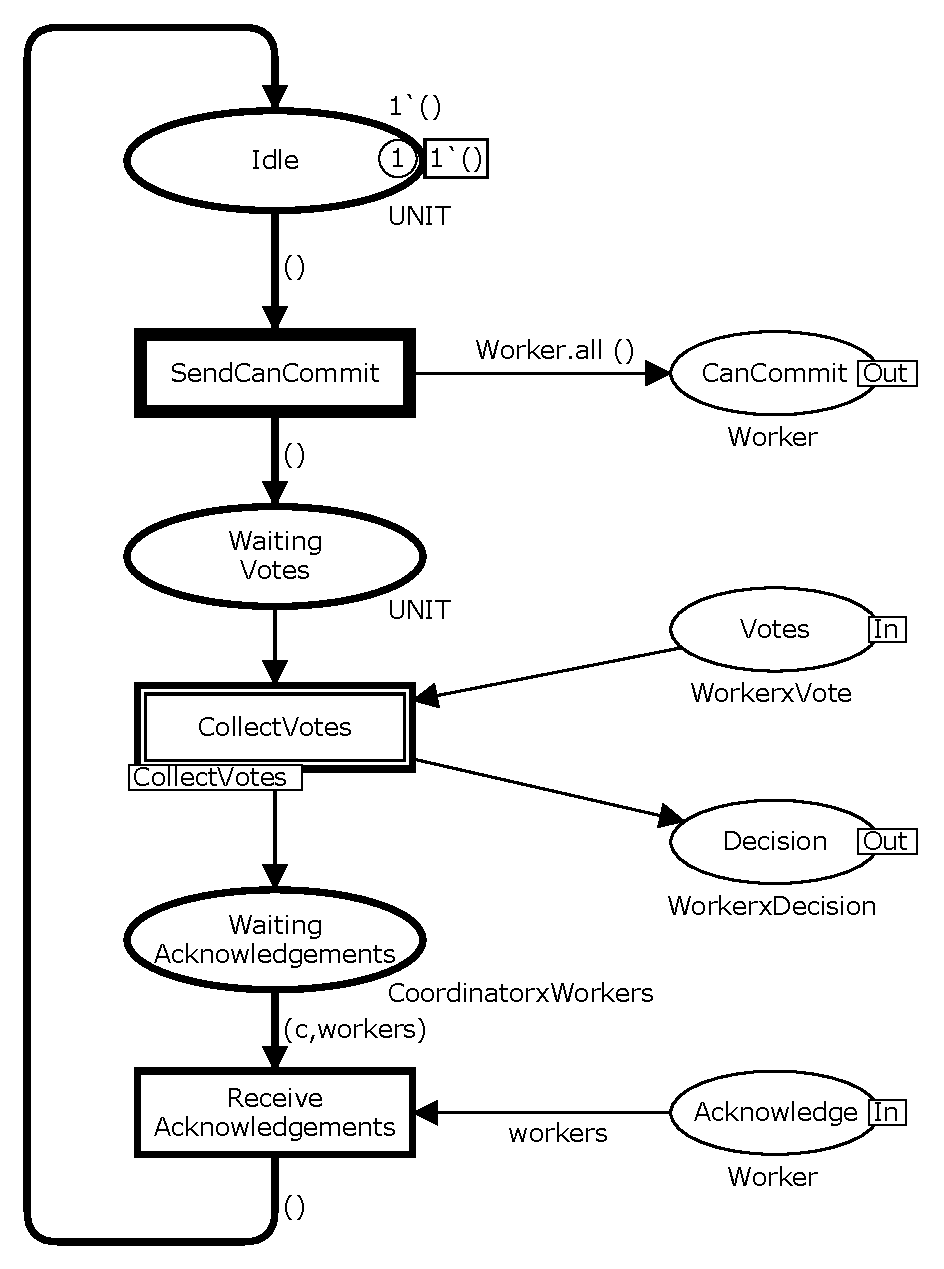
\includegraphics[width=\columnwidth]{figures/Coordinator.eps}
\caption{The Coordinator module.}
\end{figure}

\begin{figure}[t]
\centering
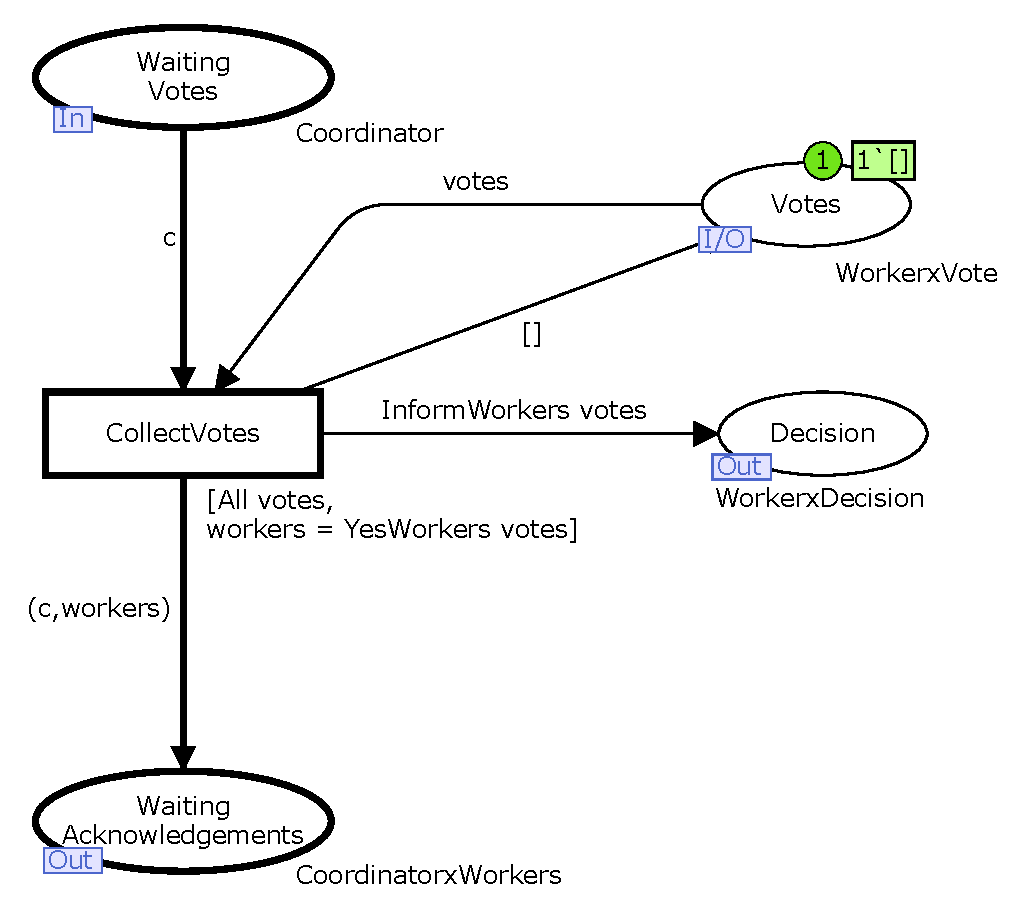
\includegraphics[width=\columnwidth]{figures/CollectVotes.eps}
\caption{The CollectVotes module.}
\end{figure}

\begin{figure}[t]
\centering
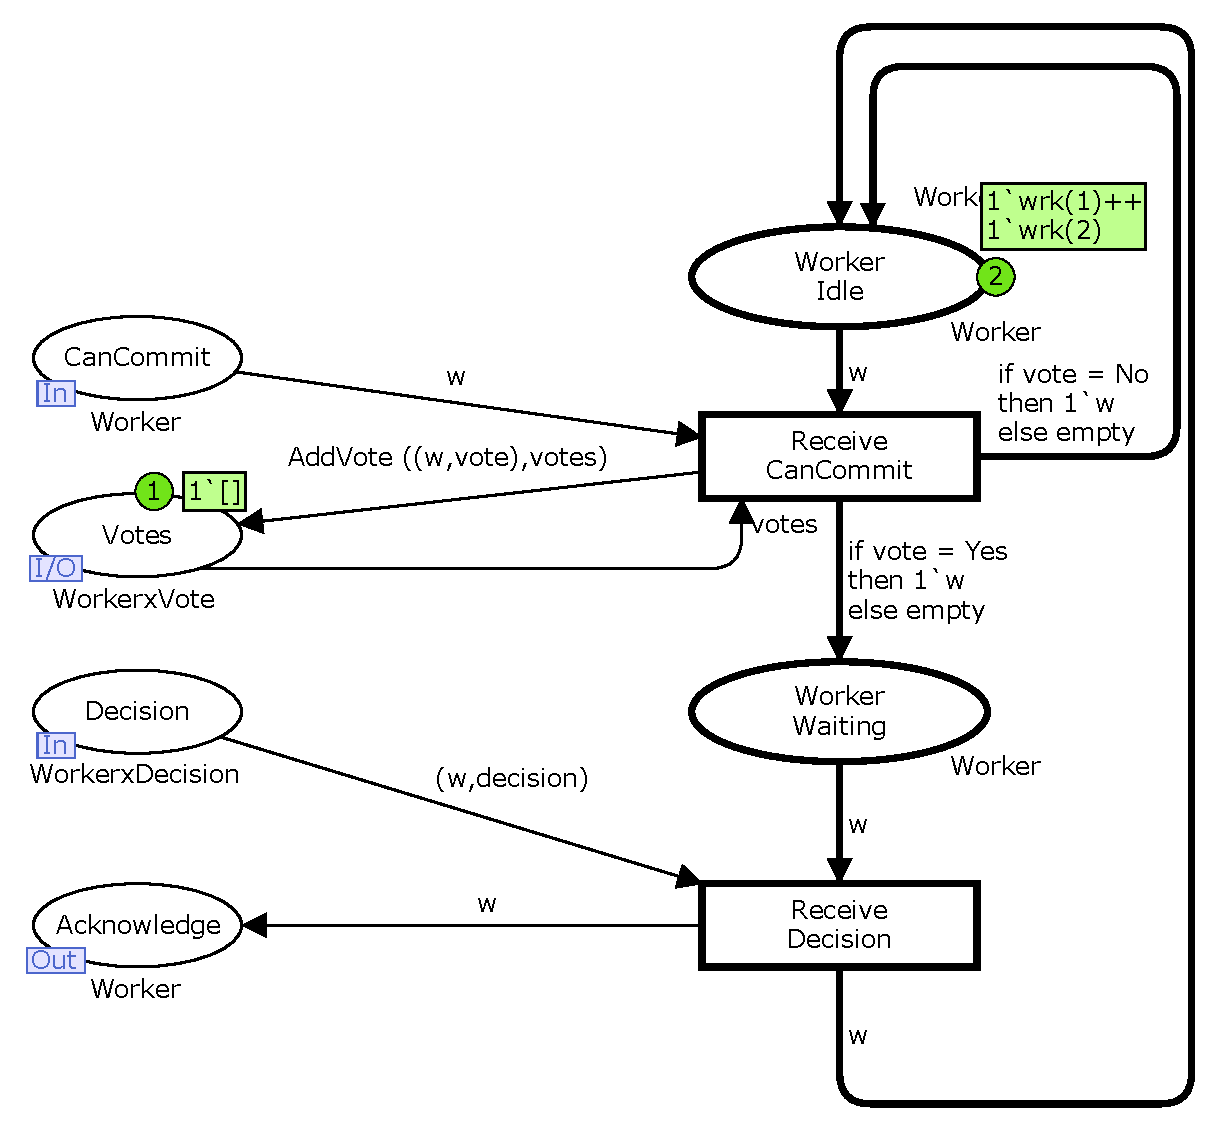
\includegraphics[width=\columnwidth]{figures/Worker.eps}
\caption{The Worker module.}
\end{figure}

\begin{figure}
\begin{verbatim}
colset INT = int;
var i : INT;

colset Coordinator = with c;
colset CoordinatorxInt = product Coordinator * INT;

colset Worker = index wrk with  1..2;
var w: Worker;

colset WorkerList = list Worker;
var workers : WorkerList;

colset CoordinatorxWorkers = product Coordinator * WorkerList;

colset Vote = with Yes | No;
var vote : Vote;

colset WorkerxVotes = product Worker * Vote;
colset WorkerxVote = list WorkerxVotes;
var votes : WorkerxVote;

colset Decision = with abort | commit;
var decision : Decision;

colset WorkerxDecision = product Worker * Decision;
\end{verbatim}
\caption{Colour sets and variable declarations.}
\end{figure}

\begin{figure}
\begin{verbatim}
val Workers = Worker.all();

fun AddVote ((w,vote),votes) = 
    sort_ms WorkerxVotes.lt ((w,vote)::votes);

fun YesWorkers votes = 
    List.map (fn (w,_) => w) 
      (List.filter (fn (w,Yes) => true 
                     | (w,No) => false) votes);

fun InformWorkers votes = 
    if (List.all (fn (_,Yes) => true 
                   | _ => false) votes)
                                            
    then List.map (fn w => (w,commit)) (YesWorkers votes)
    else List.map (fn w => (w,abort)) (YesWorkers votes);

fun All votes = List.length votes = List.length (Worker.all());
\end{verbatim}
\caption{Values and function definitions.}
\end{figure}


\section{Timed CPNs}

\section{Validation}

WILL BE BRIEF

\section{CPN Tools and Applications}

Editing, simulation, and state space exploration of CPN models is
supported by CPN Tools.

\section{Conclusions and Perspectives}

\bibliographystyle{abbrv}
\bibliography{sigproc}  % sigproc.bib is the name of the Bibliography in this case
\end{document}
